\documentclass[12pt]{article}
\usepackage{geometry}
\geometry{
    a4paper,
    left=2cm,
    right=2cm,
    top=3.0cm,
    bottom=2cm,
    headheight=73.23pt,
    headsep=0.5cm
}
\usepackage{graphicx}
\usepackage[utf8]{inputenc}
\usepackage[T1]{fontenc}
\usepackage[spanish]{babel}
\usepackage{fancyhdr}
\usepackage{lastpage}
\pagestyle{fancy}
\lhead{\raisebox{-0.25\height}{
\includegraphics[width=8cm]{img/duoc.png}}}
\rhead{Tomás Opazo \\ tom.opazo@profesor.duoc.cl \\ Sede Plaza Vespucio}
\cfoot{\thepage/\pageref*{LastPage}}

\usepackage{xcolor}
\usepackage{hyperref}
\hypersetup{
    colorlinks=true,
    linkcolor=blue,
    urlcolor=blue,
    pdftitle={Casos de Negocio EP2 --- DSY1103 Full Stack I},
    pdfauthor={Tomás Opazo},
}
\usepackage{enumitem}
\setlist[enumerate,1]{label=\arabic*.}
\setlist[enumerate,2]{label=\alph*)}

\usepackage{mdframed}
\usepackage{booktabs}
\usepackage{array}
\usepackage{colortbl}

% Recuadro de advertencia (disclaimer)
\newmdenv[
    linecolor=orange!60,
    backgroundcolor=orange!8,
    linewidth=1.2pt,
    roundcorner=4pt,
    innertopmargin=8pt,
    innerbottommargin=8pt,
    innerleftmargin=10pt,
    innerrightmargin=10pt
]{warningbox}

% Recuadro azul para el encabezado de cada caso
\newmdenv[
    linecolor=blue!40,
    backgroundcolor=blue!5,
    linewidth=1.2pt,
    roundcorner=4pt,
    innertopmargin=8pt,
    innerbottommargin=8pt,
    innerleftmargin=10pt,
    innerrightmargin=10pt
]{casobox}

\begin{document}

% ============================================================
% PORTADA
% ============================================================
\title{
    \vspace{-1cm}
    \textbf{Casos de Negocio} \\[0.4em]
    \large Evaluación Parcial 2 --- Proyecto Semestral \\[0.2em]
    \normalsize DSY1103 · Full Stack I
}
\author{Tomás Opazo \\ tom.opazo@profesor.duoc.cl}
\date{\textbf{\today}}
\maketitle
\thispagestyle{fancy}

% ============================================================
% DISCLAIMER
% ============================================================
\begin{warningbox}
\textbf{Aviso importante:} Los casos de negocio descritos en este documento son
\textbf{ficticios y de carácter exclusivamente educacional}. Las empresas
mencionadas son utilizadas únicamente como contexto de aprendizaje para que
los estudiantes practiquen el diseño e implementación de sistemas de software.
Este documento \textbf{no representa}, de ninguna manera, a las empresas
nombradas, sus productos, servicios, planes comerciales o estrategias reales.
Cualquier similitud con proyectos reales es coincidencia.
\end{warningbox}

\vspace{0.5em}

% ============================================================
% INTRODUCCIÓN
% ============================================================
\section*{Sobre este documento}

Este documento contiene los \textbf{requerimientos de negocio} para la EP2.
Cada grupo recibirá un caso distinto que define el dominio, el problema a
resolver y los módulos funcionales esperados.

Los \textbf{requerimientos técnicos} (arquitectura de microservicios, stack
tecnológico, estándares de calidad, seguridad y entrega) están definidos en
el documento complementario \textit{Directrices para Escoger Tema del Proyecto
Semestral} y aplican de igual forma a todos los casos.

\vspace{0.5em}

% ============================================================
% RÚBRICA DE EVALUACIÓN
% ============================================================
\section*{Rúbrica de evaluación}
\addcontentsline{toc}{section}{Rúbrica de evaluación}

Todos los casos son evaluados con los mismos criterios y la misma ponderación.
Cada ítem representa el \textbf{20\% de la nota final} de la EP2.

\vspace{0.5em}

\begin{center}
\renewcommand{\arraystretch}{2.0}
\begin{tabular}{
    >{\raggedright\arraybackslash}p{4.8cm}
    >{\raggedright\arraybackslash}p{8.5cm}
    >{\centering\arraybackslash}p{1.8cm}
}
\toprule
\rowcolor{blue!12}
\textbf{Ítem} & \textbf{Qué se evalúa} & \textbf{Pond.} \\
\midrule
\textbf{Arquitectura del sistema}
    & Mínimo 10 microservicios Spring Boot con responsabilidad única
      y APIs REST bajo principios RESTful (Protocolo + Dominio + Puerto +
      Ruta + Parámetros).
    & 20\% \\
\midrule
\textbf{Comunicación entre microservicios}
    & Uso de \textbf{WebClient} para llamadas sincrónicas entre al menos
      dos servicios, con consultas y validaciones cruzadas que aseguren
      la consistencia de los datos.
    & 20\% \\
\midrule
\textbf{Persistencia de datos}
    & Base de datos independiente por servicio (MySQL, PostgreSQL u Oracle),
      modelo relacional normalizado con diagrama ER, uso de DTOs y
      validaciones con Spring Boot Validation.
    & 20\% \\
\midrule
\textbf{Roles de usuario}
    & Entre 2 y 3 roles diferenciados con comportamientos y accesos
      distintos según perfil (ej.: Administrador, Cliente, Operador).
      Cada rol debe tener acciones exclusivas dentro del sistema.
    & 20\% \\
\midrule
\textbf{Funcionalidades del sistema}
    & El flujo mínimo demostrable del caso asignado se ejecuta correctamente
      de extremo a extremo en una \textit{live demo} con todos los servicios
      en funcionamiento.
    & 20\% \\
\midrule
\rowcolor{gray!10}
\textbf{Total} & & \textbf{100\%} \\
\bottomrule
\end{tabular}
\end{center}

\vspace{0.5em}
{\small\textit{El documento \textbf{Directrices para Escoger Tema del Proyecto
Semestral} define el contexto técnico general del proyecto. Los ítems marcados
en dicho documento corresponden a aspectos que \textbf{no serán evaluados en
esta instancia}.}}

% ============================================================
% ÍNDICE
% ============================================================
\tableofcontents
\newpage

% ============================================================
% CASO 1
% ============================================================
\section{Caso 1 --- Almacenes Paris: Marketplace de Mejoramiento del Hogar}
\label{caso:1}

\begin{casobox}
\textbf{Empresa (ficticia):} Almacenes Paris \hfill
\textbf{Industria:} Retail / Comercio electrónico
\end{casobox}

\begin{figure}[h]
    \centering
    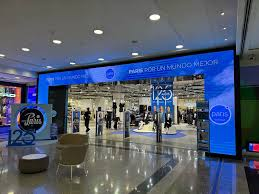
\includegraphics[width=5cm]{img/caso1_paris.jpeg}
\end{figure}

\subsection*{Contexto de negocio}

El retail tradicional funciona con un modelo de \textbf{tienda propia}: el
retailer compra mercadería a proveedores, asume el riesgo de inventario y
gana el margen entre costo y precio de venta. Un \textbf{marketplace} cambia
radicalmente esa lógica: terceros vendedores publican sus productos en la
plataforma, asumen su propio stock, y la empresa operadora cobra solo una
\textbf{comisión por venta realizada}. El resultado es que la plataforma
escala sin acumular inventario ni capital inmovilizado.

Almacenes Paris opera hoy bajo el modelo de tienda propia. La dirección ha
decidido transformar su portal en un marketplace de \textbf{mejoramiento del
hogar}, permitiendo que ferreterías, distribuidoras de pinturas e
importadores de herramientas vendan directamente a los clientes a través de
la plataforma de Paris. El desafío adicional es que la empresa ya cuenta con
\textbf{5.000 clientes registrados} en un sistema legacy que deben poder
seguir usando sus credenciales sin re-registrarse.

\noindent\textbf{Cliente histórico.}
María ingresa con su correo habitual; el sistema valida sus credenciales
contra la API legacy. Busca un taladro, elige entre ofertas de distintos
vendedores, paga y sigue el estado del despacho desde su perfil. Cuando
el producto llega defectuoso, abre un reclamo; el Administrador media la
disputa y autoriza el reembolso.

\noindent\textbf{Nuevo cliente.}
Pedro se registra, explora el catálogo de pinturas de varios vendedores,
agrega productos al carrito y completa su primera compra. Al día siguiente
recibe la notificación de despacho.

\noindent\textbf{Vendedor.}
Ferretería Cóndor completa el formulario de postulación y sube sus
documentos. El Administrador aprueba la cuenta. El vendedor publica su
catálogo, fija precios y stock; al recibir la primera orden, prepara el
despacho y marca el pedido como enviado.

\noindent\textbf{Administrador.}
Revisa solicitudes de vendedores pendientes, aprueba o rechaza con
observaciones, atiende quejas de compradores y descarga el reporte
semanal de ventas por categoría.

% ============================================================
% CASO 2
% ============================================================
\newpage
\section{Caso 2 --- Antofagasta Minerals: Gestión de Flota Minera Autónoma}
\label{caso:2}

\begin{casobox}
\textbf{Empresa (ficticia):} Antofagasta Minerals \hfill
\textbf{Industria:} Minería / Automatización industrial
\end{casobox}

\begin{figure}[h]
    \centering
    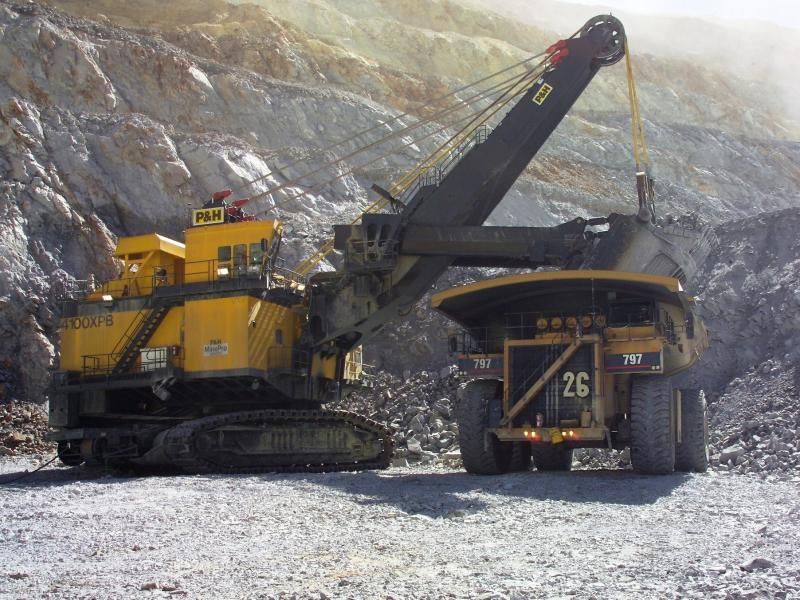
\includegraphics[width=11cm]{img/caso2_antofagasta.jpg}
\end{figure}

\subsection*{Contexto de negocio}

Antofagasta Minerals opera yacimientos de cobre a cielo abierto en el norte
de Chile. El negocio consiste en extraer mineral del rajo, transportarlo al
\textbf{chancador} para obtener concentrado de cobre exportable, y depositar
el material estéril en canchas de \textbf{relaves}. La eficiencia depende
de completar el mayor número de ciclos por turno y de que el material
correcto llegue al destino correcto: enviar mineral de alta ley a relaves
representa pérdidas millonarias. La empresa ha tomado la decisión de
\textbf{automatizar su flota de camiones}: los vehículos son ahora
autónomos ---sin conductor humano--- lo que obliga a digitalizar toda la
coordinación que antes se hacía por radio y planilla.

\noindent\textbf{Palero.}
Carlos registra su pala como operativa al iniciar turno. Los camiones
llegan autónomos; él los carga y registra el tipo de material. El sistema
asigna el destino (chancado o relaves). Cuando su pala falla, la reporta
y el sistema redistribuye las asignaciones a palas vecinas.

\noindent\textbf{Supervisor de despacho.}
Ana ve en el panel todos los camiones disponibles, en tránsito o en
mantención. Cuando el Camión 07 no reporta posición en 8 minutos, el
sistema genera una alerta; Ana lo interviene y notifica a mantención.
Al cierre del turno descarga el reporte: ciclos, toneladas a chancado y
a relaves.

\noindent\textbf{Camión autónomo (chofer virtual).}
El Camión 03 recibe la orden de ir a Pala 2, actualiza su estado a
\textit{en tránsito}, luego a \textit{cargando}, recibe el destino
\textit{relaves} y descarga. El ciclo queda registrado y el camión vuelve
a \textit{disponible}.

% ============================================================
% CASO 3
% ============================================================
\newpage
\section{Caso 3 --- Salmones Austral: Plataforma de Monitoreo de Cultivo}
\label{caso:3}

\begin{casobox}
\textbf{Empresa (ficticia):} Salmones Austral \hfill
\textbf{Industria:} Acuicultura / Salmonicultura
\end{casobox}

\begin{figure}[h]
    \centering
    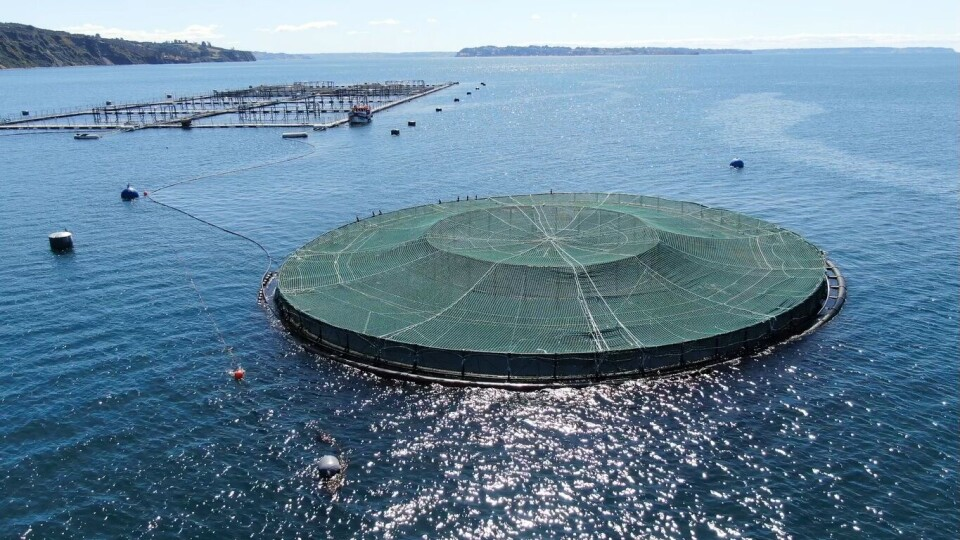
\includegraphics[width=13cm]{img/caso3_salmones.jpg}
\end{figure}

\subsection*{Contexto de negocio}

La \textbf{salmonicultura} opera en dos etapas: agua dulce, donde los peces
nacen y crecen como smolts en pisciculturas; y agua de mar, donde los smolts
se transfieren a \textbf{jaulas flotantes} en fiordos y crecen entre 12 y
18 meses hasta alcanzar el peso de cosecha. El ingreso proviene de vender
salmón procesado a mercados internacionales; el precio por kilo depende de
la calidad, las certificaciones sanitarias y el cumplimiento regulatorio
ante Sernapesca. El principal costo de producción es el alimento, medido
por el \textbf{FCR} (factor de conversión alimentaria): cuántos kilos de
alimento se necesitan para producir un kilo de salmón. Un brote del
\textbf{virus ISA} puede obligar a sacrificar un centro entero ---cientos de
miles de peces--- con pérdidas de millones de dólares y sanciones de
Sernapesca. Hoy, gran parte del monitoreo se registra en planillas físicas,
impidiendo detectar problemas a tiempo.

Salmones Austral opera varios centros en los fiordos del sur de Chile. El
desafío que se les plantea es digitalizar el monitoreo de sus jaulas:
\textbf{calidad del agua} (temperatura, oxígeno disuelto, salinidad),
mortalidad diaria, blooms de \textbf{algas nocivas} (marea roja),
tratamientos sanitarios con sus períodos de resguardo obligatorios antes
de cosecha, y gestión de la \textbf{alimentación} por jaula.

\noindent\textbf{Técnico de jaulas (Jorge).}
Cada mañana recorre las 12 jaulas en lancha, registra mortalidad y
parámetros de agua. Cuando la mortalidad de Jaula 7 sube a 0,15\% en tres
días, levanta una alerta con fotos. El veterinario recibe la notificación
desde Puerto Montt.

\noindent\textbf{Médico veterinario (Dra. Molina).}
Revisa el dashboard sanitario de todos sus centros. Diagnostica un posible
brote de SRS, ingresa el plan de tratamiento con dosis y duración, y define
30 días de resguardo. El sistema bloquea automáticamente la cosecha de esa
jaula y registra la trazabilidad del medicamento para Sernapesca.

\noindent\textbf{Supervisor de centro (Pedro).}
Cuando el monitoreo ambiental detecta un bloom de algas en el fiordo, el
sistema genera alerta crítica. Pedro suspende la alimentación en todo el
centro, verifica las redes de contención y escala al gerente. La incidencia
queda registrada con fecha, hora y acciones para el informe regulatorio.

% ============================================================
% CASO 4
% ============================================================
\newpage
\section{Caso 4 --- Karübag: Plataforma de Gestión de Reciclaje}
\label{caso:4}

\begin{casobox}
\textbf{Empresa (ficticia):} Karübag \hfill
\textbf{Industria:} Economía circular / Gestión de residuos
\end{casobox}

\begin{figure}[h]
    \centering
    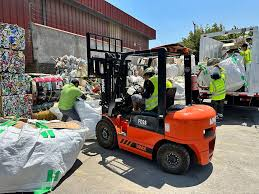
\includegraphics[width=6cm]{img/caso4_karubag.jpeg}
\end{figure}

\subsection*{Contexto de negocio}

La \textbf{economía circular del reciclaje} funciona como un mercado de dos
lados: por un lado, los clientes pagan por deshacerse de sus reciclables de
forma responsable; por otro, esos materiales se venden como
\textbf{commodities} a recicladoras ---el cartón, plástico, vidrio y metales
tienen precios de mercado que fluctúan. La clave económica está en la
\textbf{eficiencia de ruta}: cuanto más clientes se atienden por kilómetro
recorrido, menor es el costo por retiro y mayor el margen. A esto se suma
que las empresas corporativas exigen cada vez más \textbf{certificados de
reciclaje} para sus informes de sustentabilidad (ESG), convirtiéndolos en
un activo tan valioso como el material mismo.

Karübag nació en Santiago con ese modelo y se expandió a cuatro regiones
con más de 3.000 clientes activos. Esa expansión rápida generó una
\textbf{crisis operacional silenciosa}: rutas gestionadas en planillas,
clientes coordinados por WhatsApp, certificados emitidos a mano en Word,
y sin trazabilidad del material desde el retiro hasta la recicladora final.
La dirección necesita una plataforma que ordene y automatice el crecimiento.

\noindent\textbf{Cliente residencial (Catalina).}
Se suscribió al plan básico; cada lunes deja su bolsa en la entrada.
Desde la plataforma ve su historial de retiros y kilos reciclados por
tipo, y descarga su Certificado de Impacto. Cuando el operador no pasa,
reporta el retiro fallido y el sistema lo reagenda automáticamente.

\noindent\textbf{Cliente corporativo.}
Una constructora con tres oficinas gestiona sus retiros desde un panel
centralizado, configura la frecuencia de cada sede y descarga al cierre
del trimestre el \textbf{Certificado de Reciclaje} con kilos por material,
que adjunta a su reporte ESG.

\noindent\textbf{Operador de ruta (Carlos).}
Ve su ruta del día con 28 paradas ordenadas. En cada parada registra los
kilos por tipo de material. Si el cliente no deja material, lo marca como
\textit{ausente}; eso excluye el retiro de la facturación del mes y deja
el registro disponible para la supervisora de planta antes de que llegue
el camión.

% ============================================================
% CASO 5
% ============================================================
\newpage
\section{Caso 5 --- UNACESS: Red Nacional de Derivación en Salud Sexual}
\label{caso:5}

\begin{casobox}
\textbf{Organización (ficticia):} UNACESS --- Unidad de Atención y Control en Salud Sexual
\hfill \textbf{Industria:} Salud pública
\end{casobox}

\begin{figure}[h]
    \centering
    
\includegraphics[width=11cm]{img/caso5_unacess.jpg}
\end{figure}

\subsection*{Contexto de negocio}

En Chile, ciertas infecciones de transmisión sexual (ITS) son
\textbf{enfermedades de notificación obligatoria}: cualquier profesional de
salud que detecte un caso está legalmente obligado a reportarlo a la
autoridad sanitaria. Sin embargo, el estigma social asociado a estas
enfermedades hace que muchos pacientes eviten el sistema de salud si no
perciben confidencialidad. Las \textbf{UNACESS} (Unidades de Atención y
Control en Salud Sexual) existen para resolver esta tensión: ofrecen
atención especializada, \textbf{gratuita y confidencial}, independiente del
tramo de salud o la previsión del paciente. El desafío operacional es que el
sistema debe conectar una red heterogénea ---desde hospitales regionales
hasta postas rurales con un solo funcionario--- y canalizar casos hacia
UNACESS de forma ágil y discreta. La \textbf{protección del dato clínico}
es un requisito crítico: un diagnóstico de ITS que se filtre puede destruir
la vida laboral y social de una persona.

La UNACESS de Antofagasta atiende ITS como VIH, sífilis, gonorrea y
hepatitis B/C. Su equipo de dermatólogos y matronas recibe pacientes
derivados desde cualquier establecimiento de salud del país. Hoy, las
derivaciones llegan por teléfono, correo o en papel, sin trazabilidad ni
seguimiento centralizado. Necesitan un sistema que digitalice toda esa
cadena de referencia, desde la detección hasta el alta, sin comprometer
la privacidad de los pacientes.

\noindent\textbf{Reportador --- Enfermera de posta rural (Macarena).}
En una visita de terreno en una localidad alejada, Macarena detecta un
caso con signos compatibles con una ITS. No puede diagnosticar ni tratar
localmente. Abre el sistema, registra al paciente solo con su RUT y
genera una derivación con código anónimo. El paciente recibe un mensaje
neutro: ``tiene una cita de salud pendiente en UNACESS''. Macarena
\textbf{no tiene acceso al diagnóstico final}; solo puede ver si la
derivación fue aceptada y atendida.

\noindent\textbf{Paciente.}
Recibe el mensaje, accede al portal con su RUT y un PIN personal,
confirma la cita y asiste. Tras la consulta, su perfil muestra su plan
de tratamiento y el calendario de controles. El sistema \textbf{nunca
incluye el nombre de la enfermedad} en notificaciones ni correos; toda
la información clínica solo es visible dentro de la ficha, con acceso
restringido al equipo tratante.

\noindent\textbf{Profesional UNACESS --- Matrona Claudia.}
Cada mañana revisa la cola de derivaciones entrantes. Acepta al paciente
referido desde Calama, crea su ficha clínica, registra el diagnóstico
confirmado y asigna el protocolo de tratamiento. Programa los controles
de seguimiento. Cuando el paciente falta a dos controles consecutivos,
el sistema le genera una alerta para intentar recontacto. Al final del
mes, exporta el reporte epidemiológico anónimo para el Ministerio de Salud.

% ============================================================
% CASO 6
% ============================================================
\newpage
\section{Caso 6 --- DGAC: Plataforma Nacional de Gestión de Drones}
\label{caso:6}

\begin{casobox}
\textbf{Organización (ficticia):} DGAC --- Dirección General de Aeronáutica Civil
\hfill \textbf{Industria:} Aviación civil / Regulación
\end{casobox}

\begin{figure}[h]
    \centering
    
\includegraphics[width=13cm]{img/caso5_dgac.jpg}
\end{figure}

\subsection*{Contexto de negocio}

El espacio aéreo es un recurso compartido y regulado. En Chile, la DGAC
administra el espacio aéreo bajo las normas DAN~151 y DAN~91: los drones
(o RPA, aeronaves pilotadas remotamente) requieren piloto certificado,
aeronave registrada, seguro de responsabilidad civil y, para vuelos en zonas
pobladas, autorización de la propia DGAC. El problema estructural es que la
DGAC \textbf{carece de capacidad real de fiscalización en terreno}: los drones
son pequeños, silenciosos y operan en todo el país simultáneamente. La
estrategia elegida no es la sanción, sino la \textbf{utilidad}: si el
sistema le sirve genuinamente a cada actor ---piloto, empresa proveedora,
empresa mandante--- el cumplimiento se vuelve la opción natural.

El negocio de los drones comerciales en Chile abarca mapeo de terrenos
mineros, inspección de líneas eléctricas, fotografía inmobiliaria,
agricultura de precisión y apoyo a emergencias. El flujo típico es:
la \textbf{empresa mandante} (la que necesita el servicio) contrata a una
\textbf{empresa proveedora} (que tiene la flota y los pilotos certificados),
quien asigna un \textbf{piloto} y una aeronave al trabajo. El sistema debe
hacer visible toda esa cadena: quién vuela, qué aeronave, dónde, cuándo
y para quién.

\noindent\textbf{Piloto (Rodrigo).}
Rodrigo es piloto freelance certificado por la DGAC. La empresa eléctrica lo
contrató para inspeccionar una línea de alta tensión en la región del Maule.
Antes del vuelo, crea el plan de vuelo en el sistema: ubicación GPS del
corredor, fecha, altitud máxima y aeronave asignada. El sistema verifica
automáticamente que su certificado esté vigente, que el dron tenga seguro
activo y que la zona no esté restringida. La empresa mandante recibe la
notificación. Después del vuelo, Rodrigo registra el cierre del plan con la
duración real y cualquier incidencia. El sistema genera el bitácora digital
firmado.

\noindent\textbf{Empresa proveedora (DroneChile SpA).}
El administrador de DroneChile gestiona su flota de 12 aeronaves y 6 pilotos.
El sistema le alerta cuando el certificado de un piloto vence en 30 días o
cuando el seguro de una aeronave está próximo a expirar, antes de que pueda
ocurrir un vuelo sin cobertura. Al cierre del mes, descarga el reporte de
operaciones de todos sus pilotos para facturar a sus clientes.

\noindent\textbf{Empresa mandante (constructora).}
La jefa de proyectos tiene visibilidad de todos los vuelos contratados sobre
sus faenas: puede ver qué piloto, con qué aeronave y en qué horario se
realizará cada operación. Si detecta un vuelo no autorizado sobre su
propiedad, puede reportarlo como incidencia. Al término del proyecto,
descarga el historial completo para su archivo legal.

\noindent\textbf{DGAC (inspector).}
El inspector accede al mapa nacional de vuelos planificados y activos,
filtrable por región, fecha y tipo de operación. Revisa los reportes de
incidencias ciudadanas (vecinos que reportan drones no identificados).
Puede consultar el historial de cualquier piloto o aeronave y generar
estadísticas trimestrales: cuántos vuelos se realizaron en zonas urbanas,
cuántos incidentes se reportaron y cuál es la distribución regional de la
actividad.

% ============================================================
% CASO 7
% ============================================================
\newpage
\section{Caso 7 --- CONAF: Coordinación de Emergencias por Incendios Forestales}
\label{caso:7}

\begin{casobox}
\textbf{Organización (ficticia):} CONAF --- Corporación Nacional Forestal
\hfill \textbf{Industria:} Gestión de emergencias / Sector público
\end{casobox}

\begin{figure}[h]
    \centering
    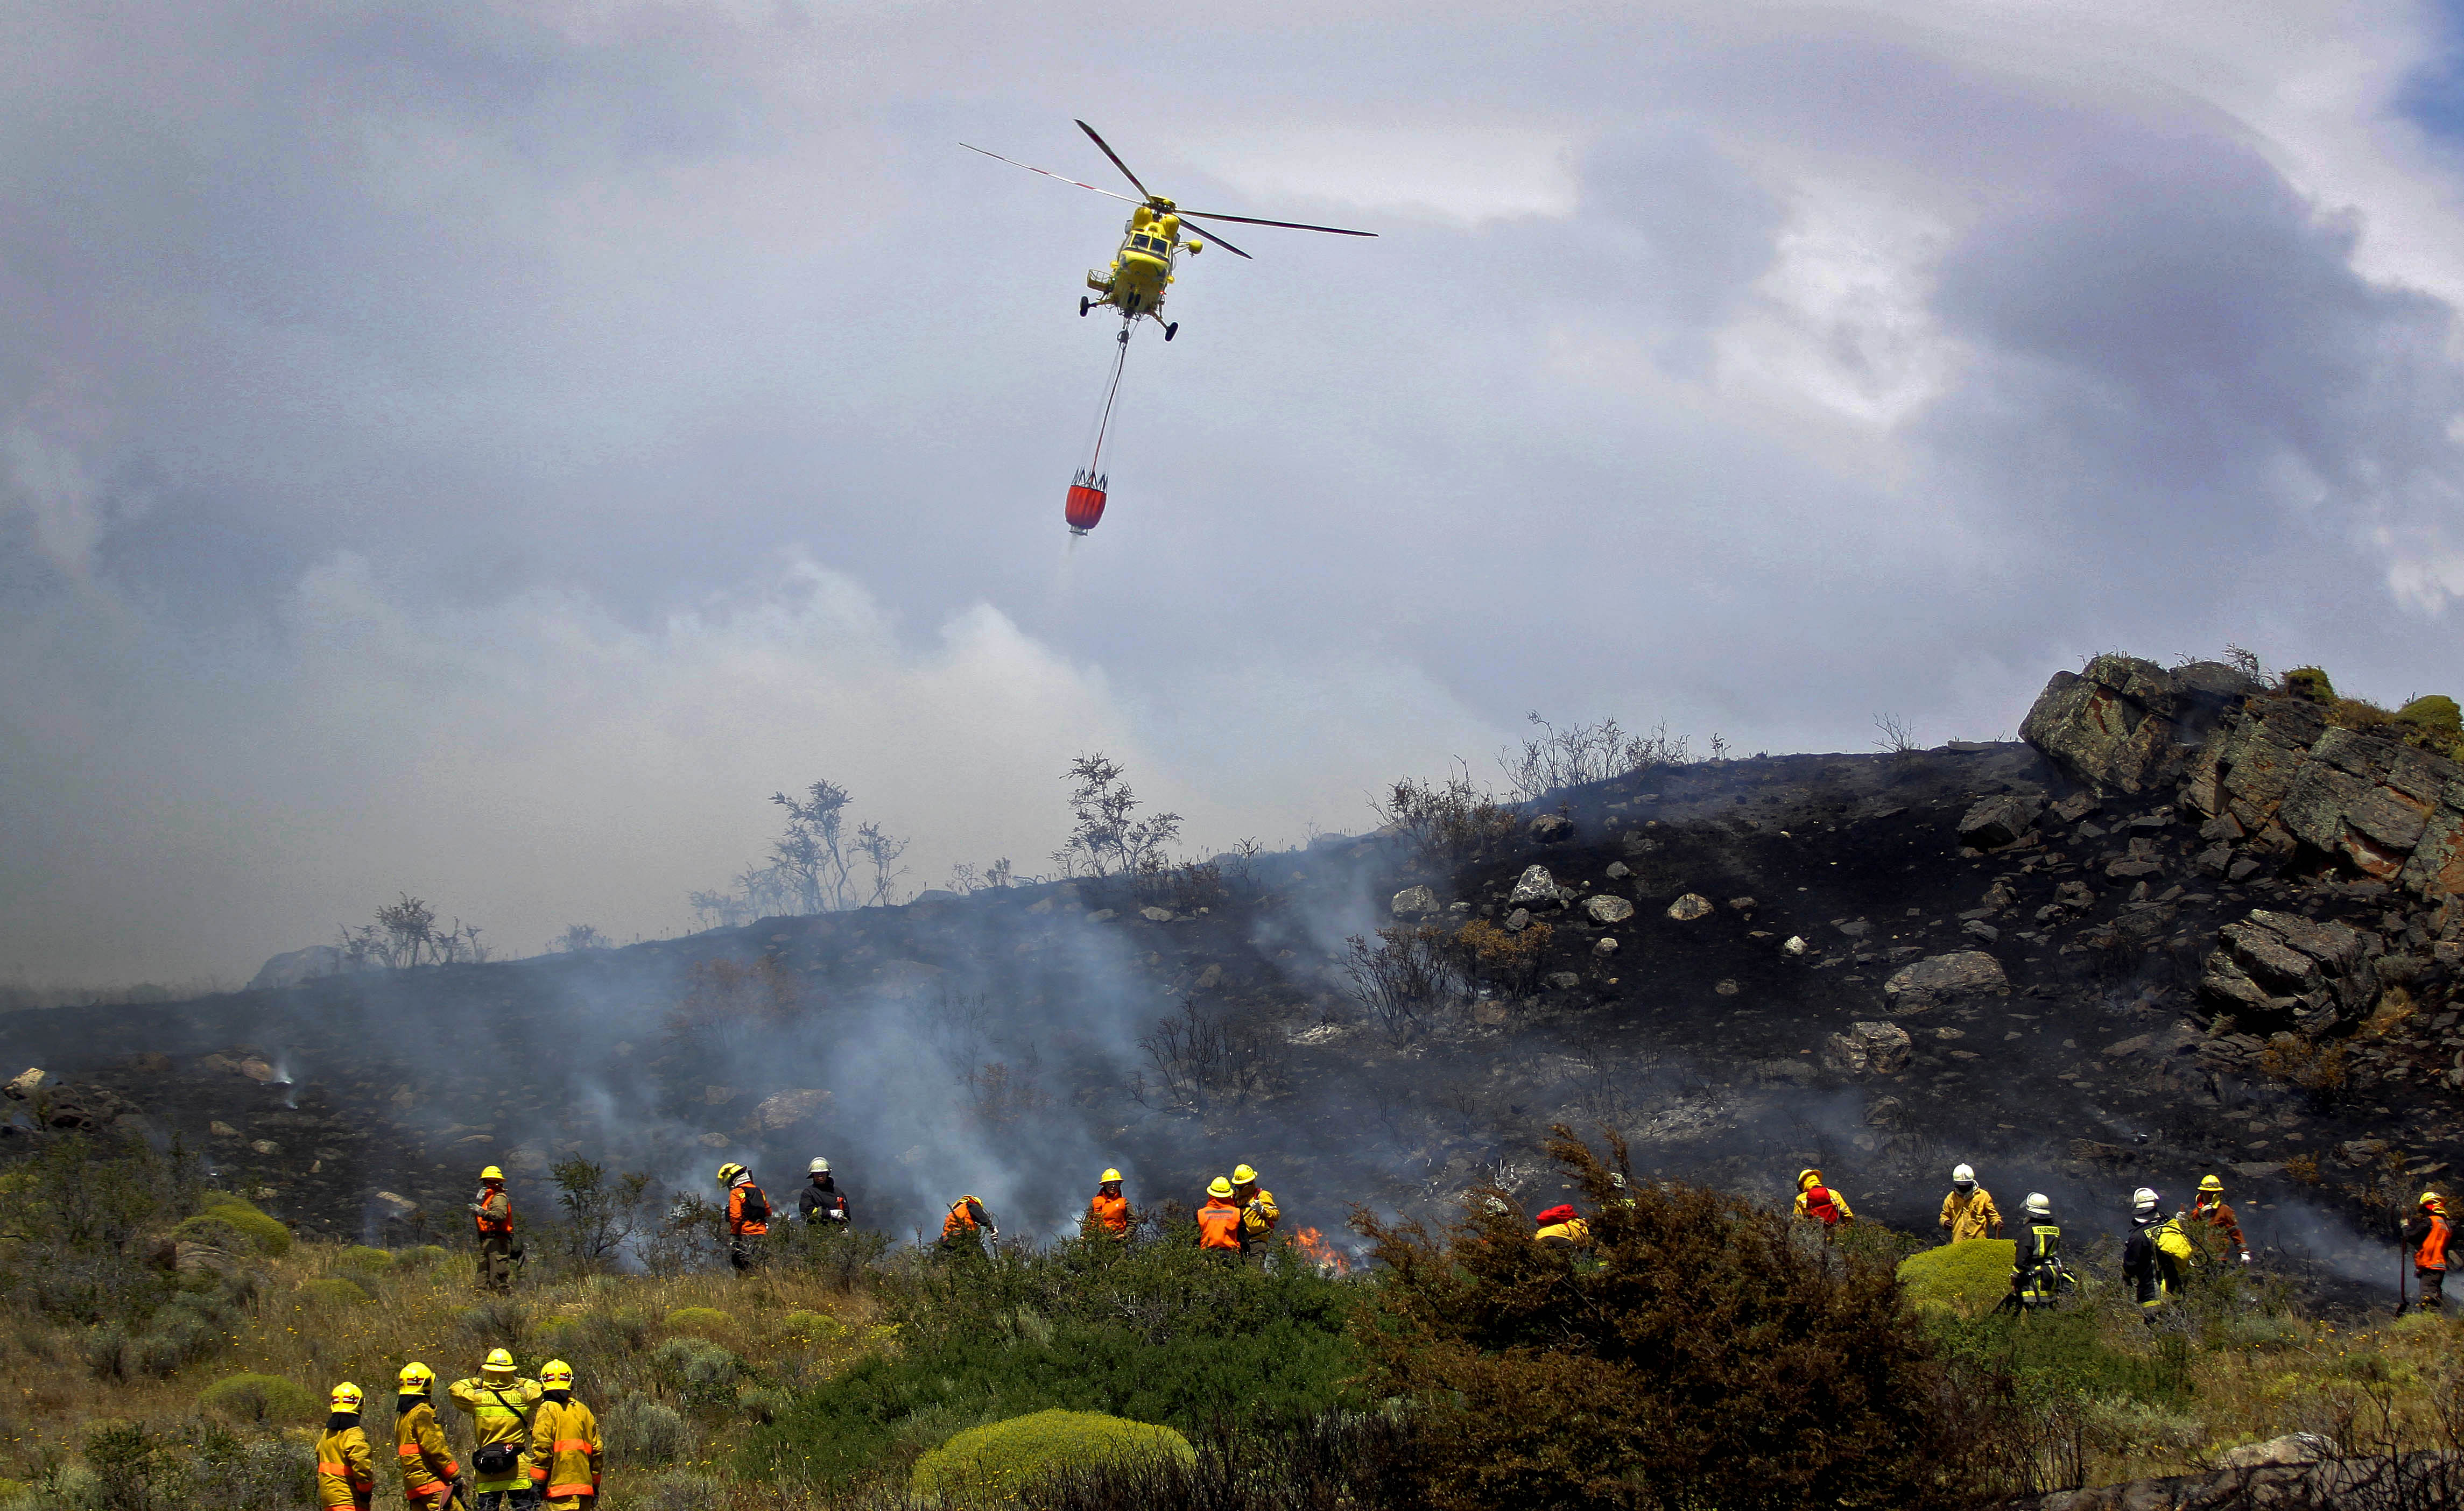
\includegraphics[width=12cm]{img/caso7_conaf.jpg}
\end{figure}

\subsection*{Contexto de negocio}

Chile padece incendios forestales devastadores por la combinación de su clima
mediterráneo, extensas plantaciones de pino y eucaliptos, y temporadas de
calor extremo. La temporada 2017 quemó más de 500.000 hectáreas en el Maule
y el Biobío; la de 2024 fue una de las más mortales de las últimas décadas.
CONAF es el organismo responsable de la respuesta, y opera como una logística
militar: recursos escasos ---\textbf{brigadas terrestres} (cuadrillas de
10--20 personas con herramientas manuales), \textbf{aviones cisterna},
\textbf{helicópteros con balde} y \textbf{camiones aljibe}--- que deben
distribuirse en tiempo real entre múltiples \textbf{frentes de fuego}
activos simultáneamente. Un error de priorización puede significar que un
frente menor consuma recursos mientras un incendio mayor avanza hacia una
comunidad. La coordinación se hace hoy con radio y planilla física; la
demora en la información tiene costes medidos en hectáreas y vidas.

\noindent\textbf{Coordinador CONAF (Roberto).}
Roberto supervisa el turno desde el centro regional en Talca. Un martes de
enero, tres focos se activan en dos horas por viento puelche. En el panel
ve sus 8 brigadas (6 activas, 2 en descanso), 2 aviones cisterna (uno en
mantención) y 4 camiones aljibe. Asigna la brigade más cercana al foco que
amenaza la comunidad de Pencahue, solicita apoyo aéreo al foco mayor y
redirige un camión aljibe al punto de abastecimiento de agua. Cada hora
registra el avance de la línea de defensa y el estado del personal. A las
18:00 genera el Parte Diario para las autoridades.

\noindent\textbf{Brigadista terrestre (Felipe).}
Su brigada recibe la orden de contener el flanco este de un incendio en
pleno monte nativo. El sistema le muestra el objetivo táctico y la posición
de las brigadas vecinas. Al cortar 600m de línea de defensa, el viento rola
y el fuego salta; Felipe reporta la nueva posición del frente y solicita
apoyo aéreo. Tras 12 horas en terreno, su brigada rota y él registra el
trabajo ejecutado, estado de la tripulación y herramientas utilizadas.

\noindent\textbf{Municipio afectado (alcaldesa de Constitución).}
La alcaldesa reporta que dos predios del sector cordillerano están en riesgo
y que 30 familias han sido evacuadas. El sistema recibe la alerta con
georreferencia y número de personas afectadas, y la eleva a CONAF regional.
Puede ver en tiempo real si se han asignado recursos a su territorio. Al
cierre del incidente, descarga el expediente completo para los trámites de
seguro y reconstrucción.

% ============================================================
% CASO 8
% ============================================================
\newpage
\section{Caso 8 --- Caleta Pesquera: Gestión de Subasta Artesanal}
\label{caso:8}

\begin{casobox}
\textbf{Empresa (ficticia):} Caleta Lo Abarca \hfill
\textbf{Industria:} Pesca artesanal / Acuicultura costera
\end{casobox}

\begin{figure}[h]
    \centering
    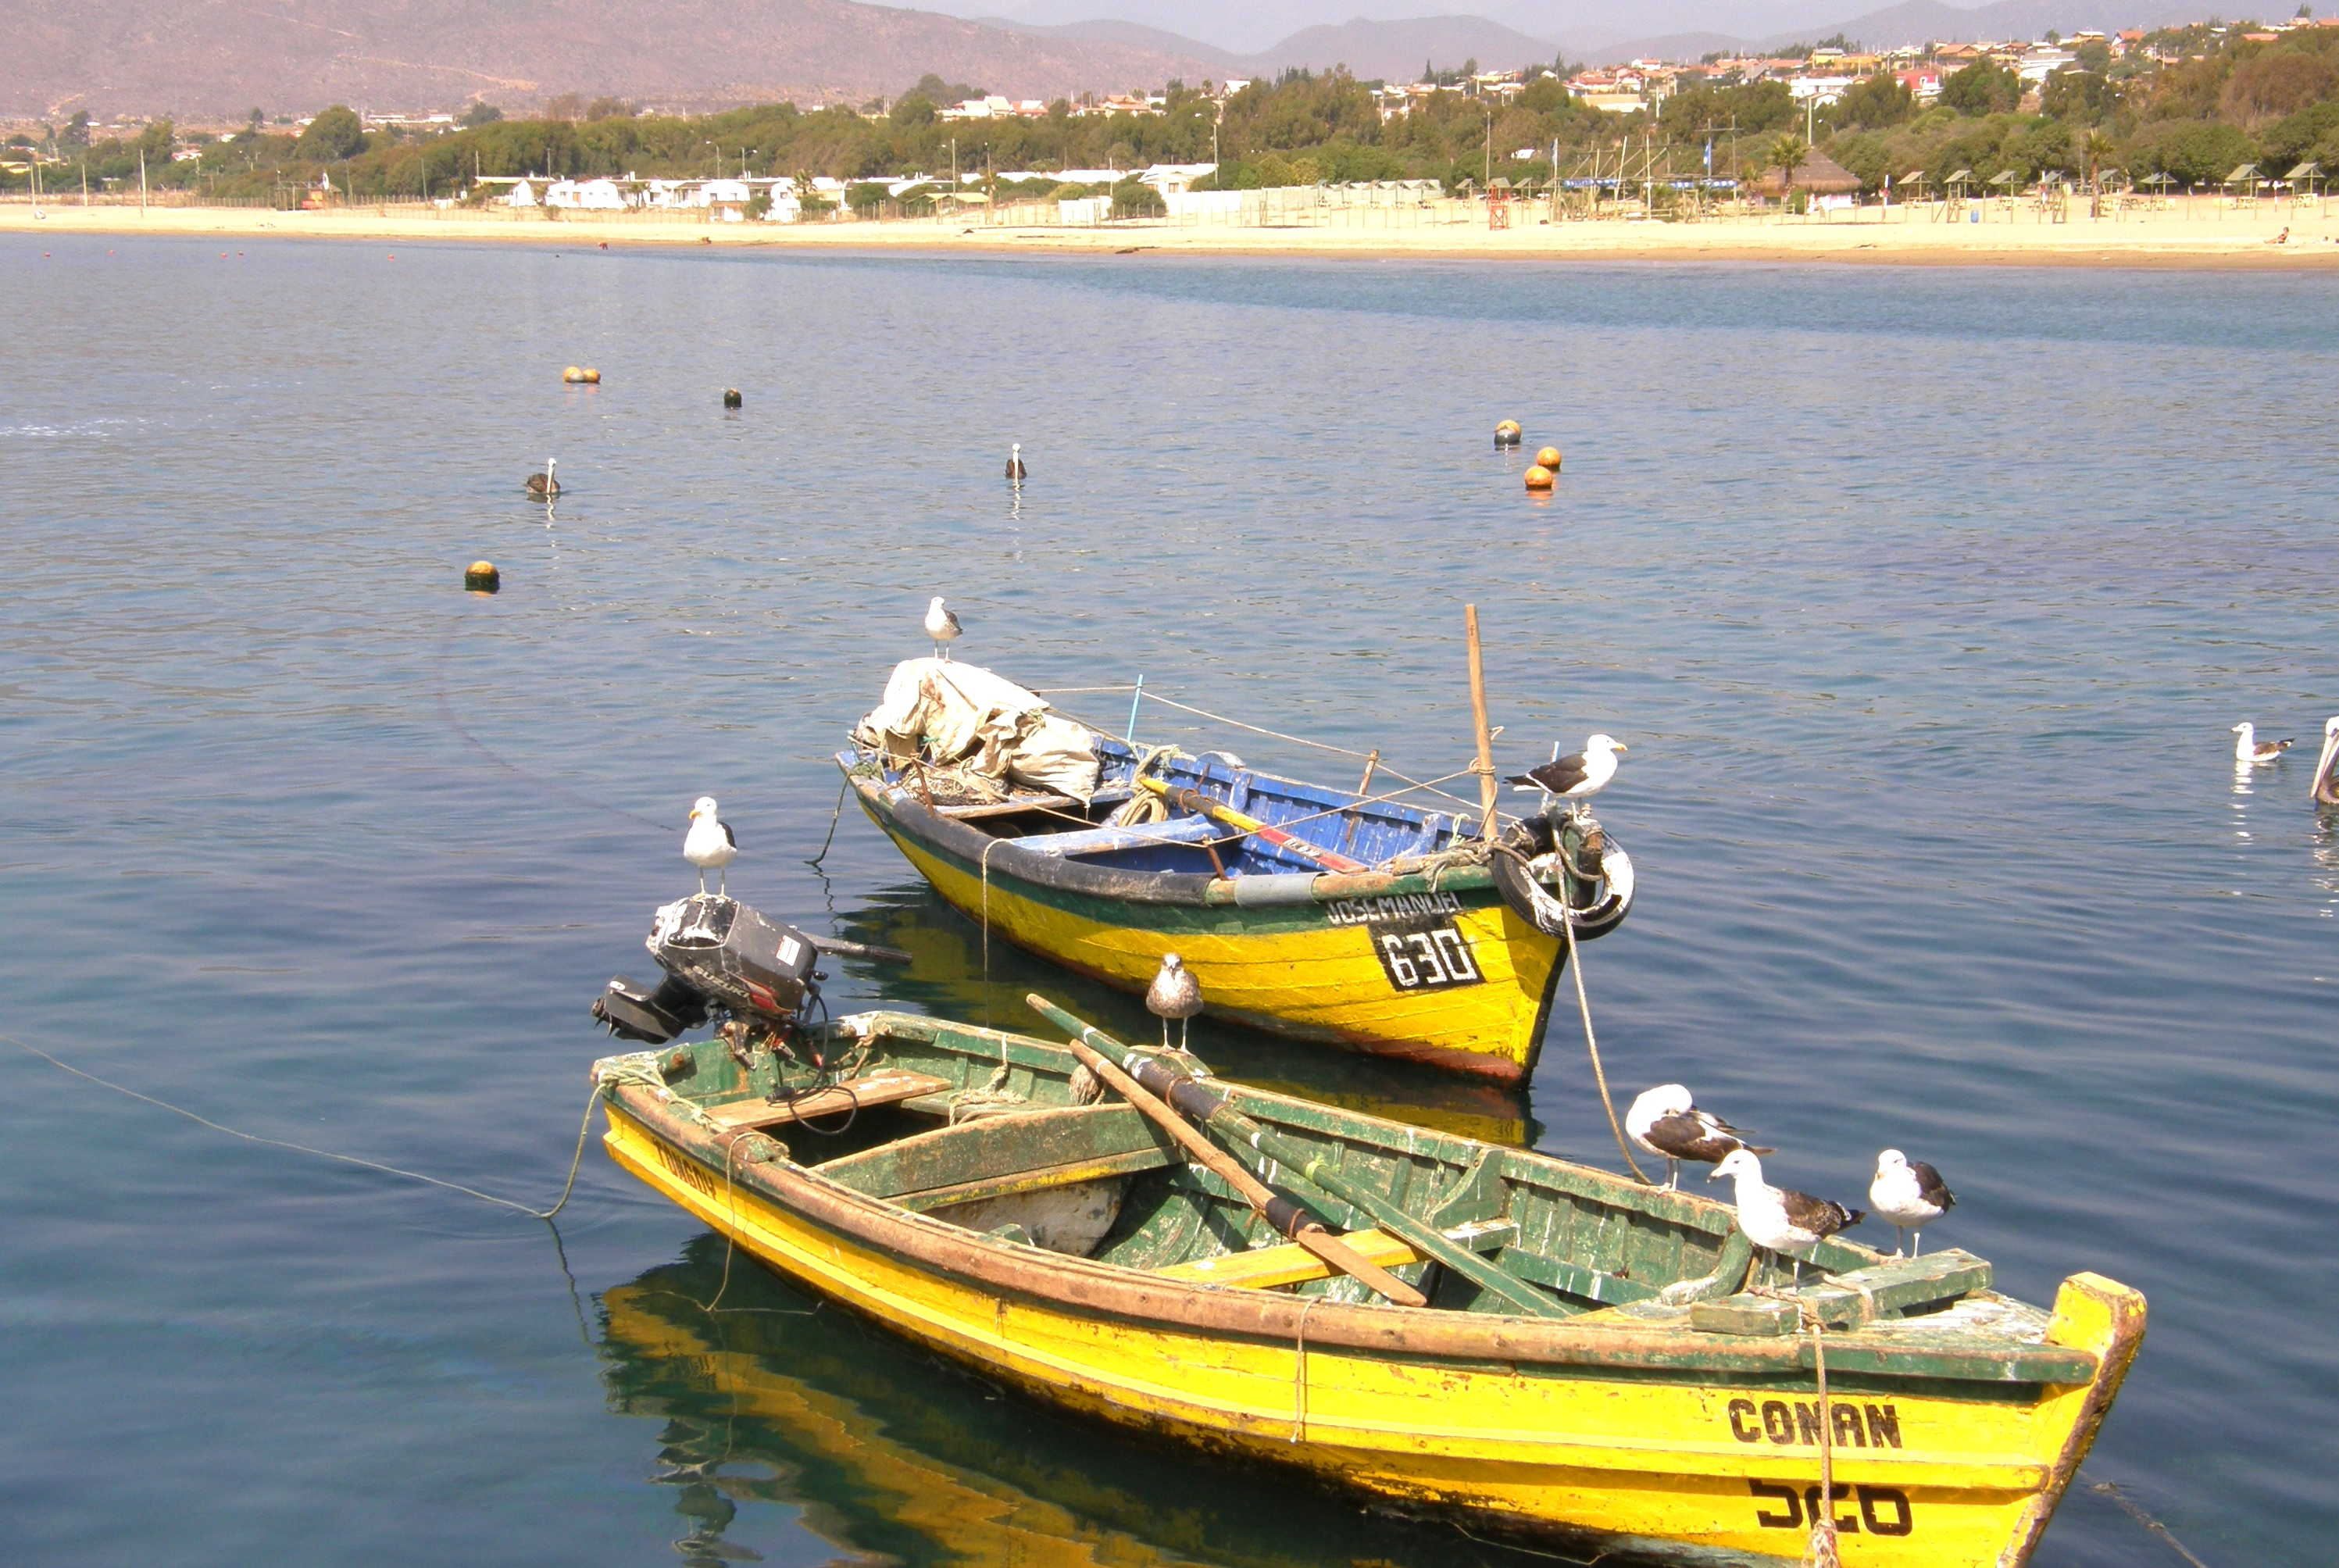
\includegraphics[width=12cm]{img/caso8_caleta.jpg}
\end{figure}

\subsection*{Contexto de negocio}

Chile posee más de 6.000 km de costa bañada por la Corriente de Humboldt,
una de las más ricas en biomasa marina del planeta. La \textbf{pesca
artesanal} se diferencia de la industrial por el tamaño de la embarcación
(menos de 18 m) y la zona de pesca (hasta 5 millas de la costa). Los
pescadores se organizan en sindicatos y operan desde \textbf{caletas}:
pequeños puertos con bodega frigorífica, grúa de descarga y espacio de
subasta. El flujo diario es el siguiente: los botes regresan al amanecer
con la captura, que es pesada en balanza certificada, registrada ante
\textbf{Sernapesca} (que controla cuotas por especie y zona para evitar
la sobreexplotación), y luego \textbf{subastada} al mejor postor entre los
compradores registrados ---restaurantes, pescaderías, procesadoras de
exportación. El precio varía por especie, calidad y oferta del día. El
pescador cobra la venta menos el \textbf{porcentaje de la caleta} (entre
6\% y 10\%). Sernapesca puede suspender la pesca de una especie sin previo
aviso si la cuota anual se agota; la caleta debe reflejarlo de inmediato.

\noindent\textbf{Pescador artesanal (Don Segundo).}
Llega a las 5:30 am con 80 kg de congrio y 30 kg de lenguado. Registra su
llegada con su licencia y el ID de su bote. El pesador ingresa los kilos en
el sistema, que verifica automáticamente que la especie y cantidad estén
dentro de su cuota. El lote se pone en subasta. A las 8:00 am Don Segundo
ve en el panel que su congrio se vendió a \$3.200/kg y el lenguado a
\$2.800/kg. El neto ---descontado el 8\% de la caleta--- queda disponible
en su estado de cuenta.

\noindent\textbf{Compradora (restaurante).}
Valentina compra dos veces por semana. La tarde anterior ingresa órdenes de
compra con precio máximo por especie: hasta 100 kg de congrio a máximo
\$3.500/kg. En la mañana, el sistema la notifica de las compras exitosas y
del horario de retiro en bodega. Si es superada en la subasta, puede ajustar
su oferta para el siguiente lote.

\noindent\textbf{Administrador de caleta.}
Abre la jornada de subasta, gestiona los lotes a medida que llegan los botes
y supervisa la bodega frigorífica. Al mes siguiente genera los liquidaciones
de pago a cada pescador, el reporte Sernapesca de especies y volúmenes
transados, y el estado de ocupación de los puestos de amarre. Cuando
Sernapesca decreta veda para una especie, activa el bloqueo en el sistema
y notifica al sindicato.

% ============================================================
% CASO 9
% ============================================================
\newpage
\section{Caso 9 --- APR La Esperanza: Cooperativa de Agua Potable Rural}
\label{caso:9}

\begin{casobox}
\textbf{Organización (ficticia):} APR La Esperanza \hfill
\textbf{Industria:} Agua potable rural / Cooperativismo
\end{casobox}

\begin{figure}[h]
    \centering
    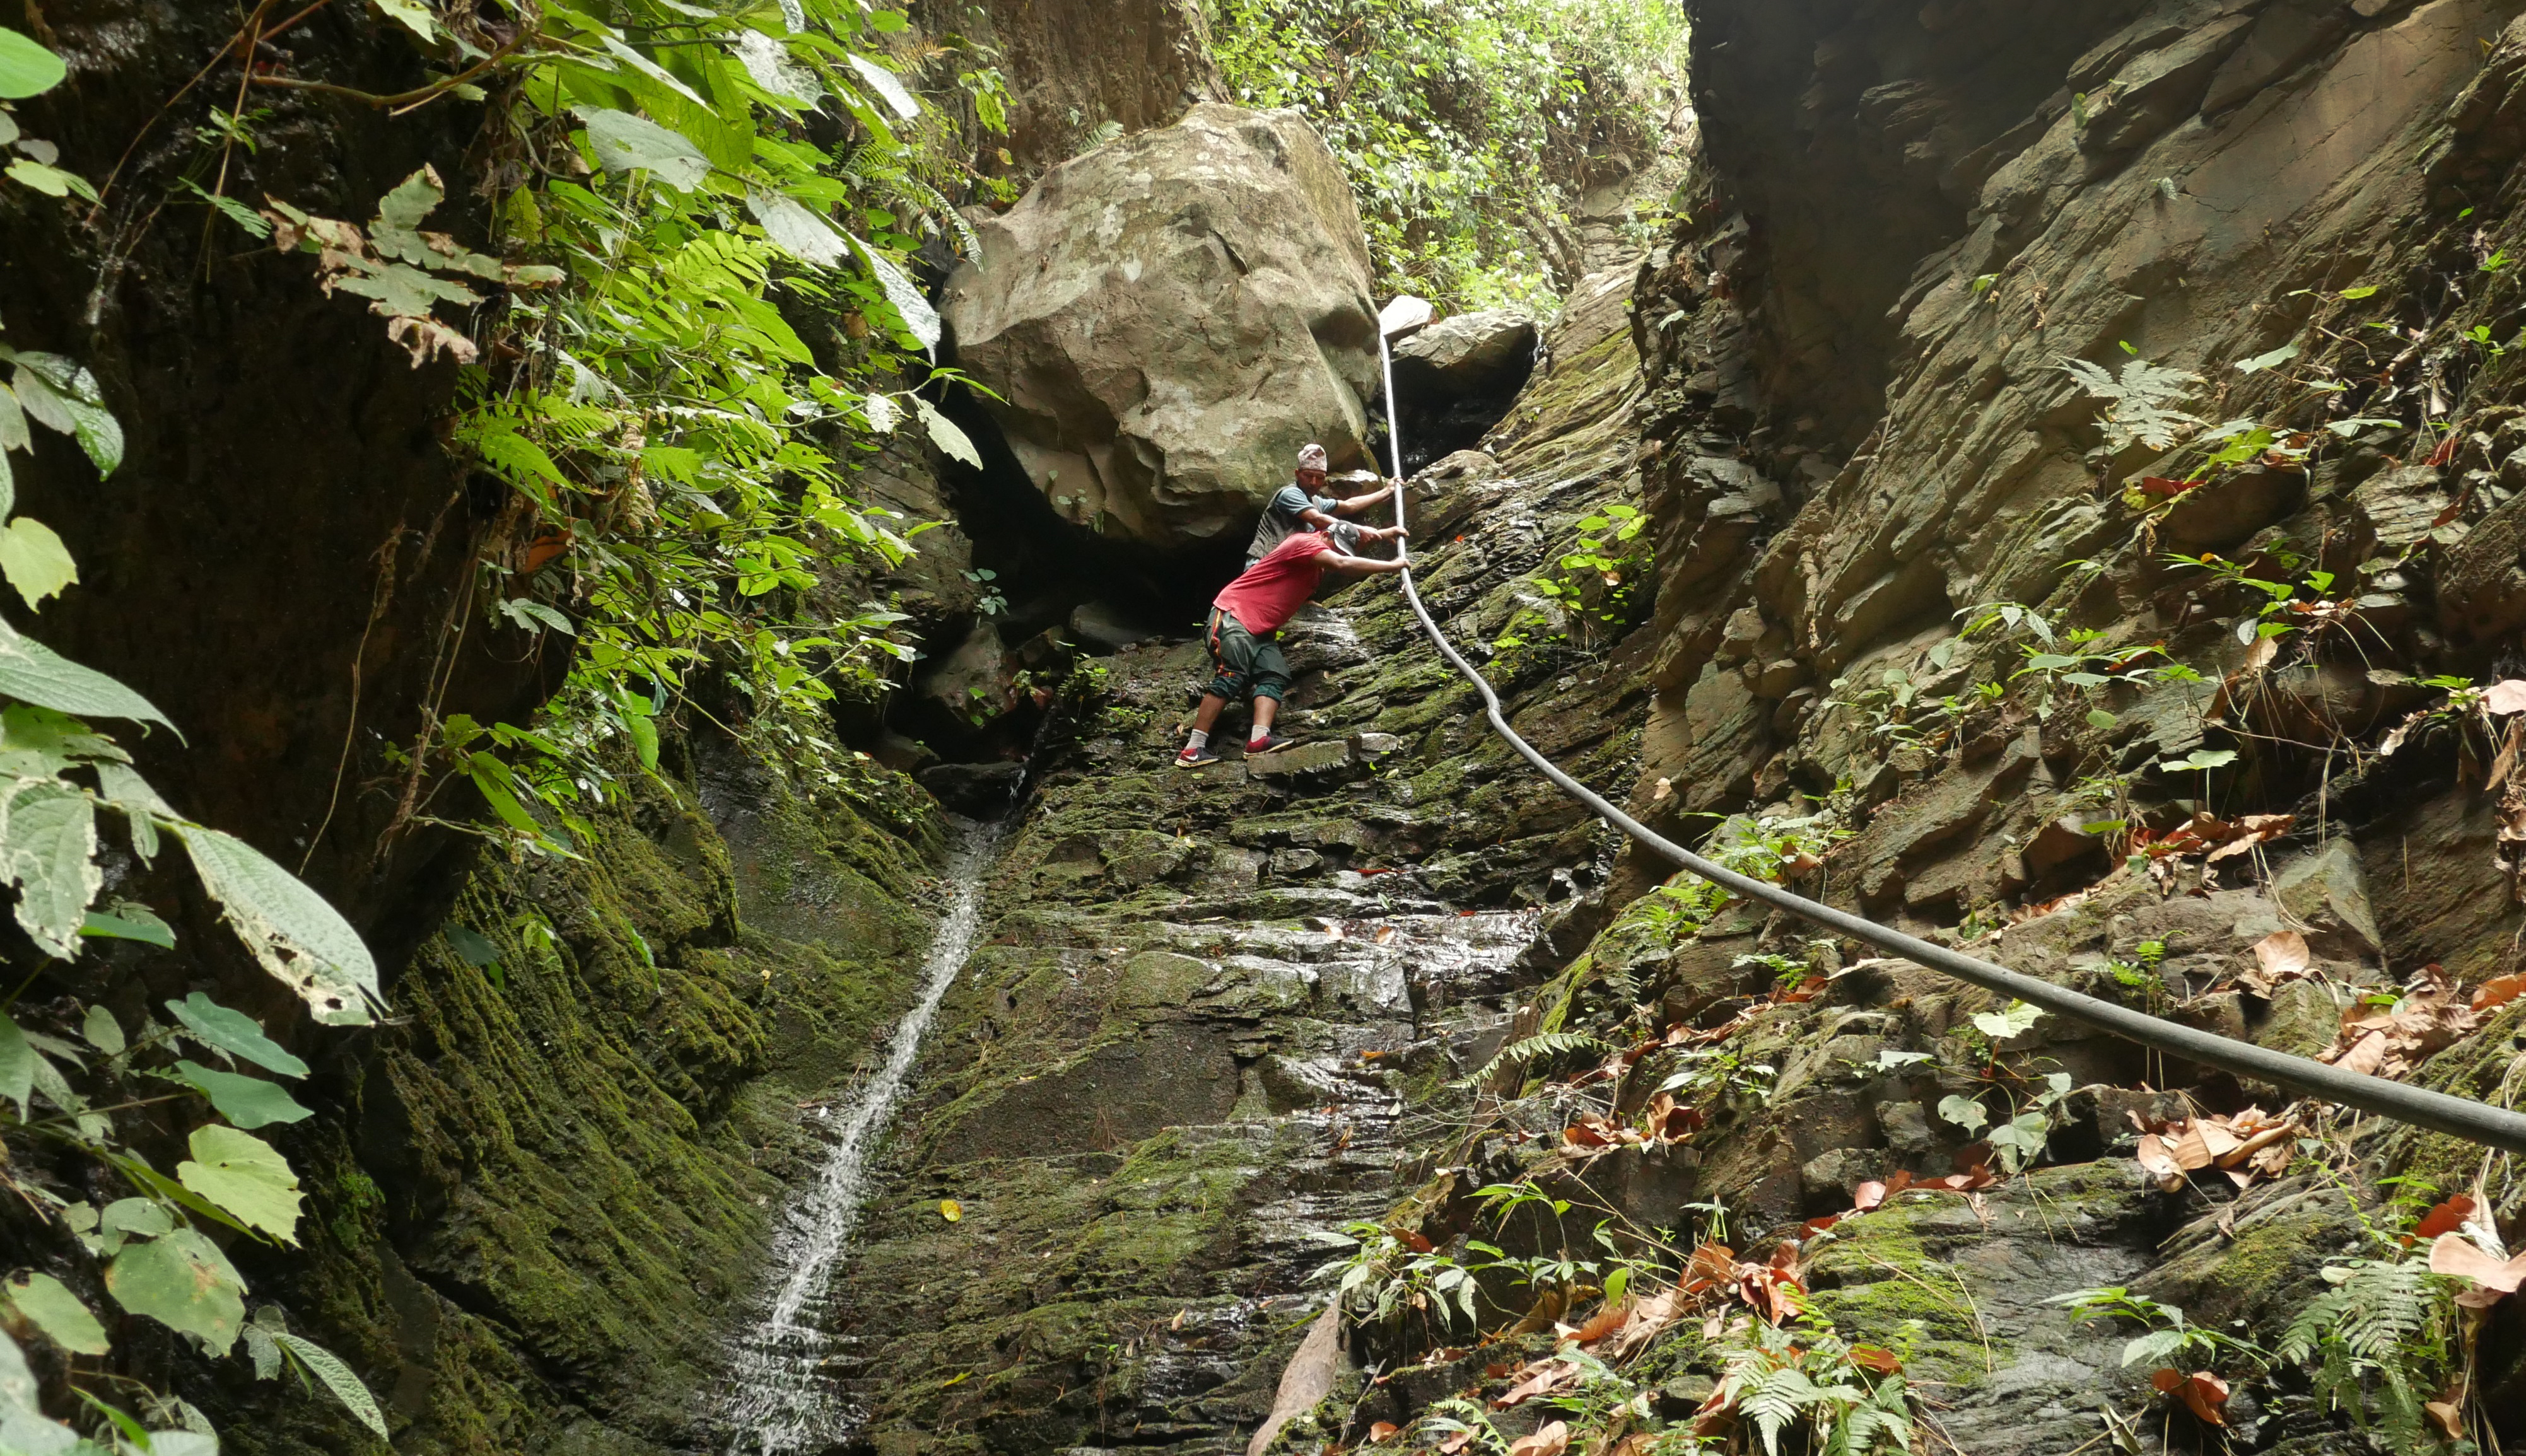
\includegraphics[width=12cm]{img/caso9_apr.jpg}
\end{figure}

\subsection*{Contexto de negocio}

Cerca del 10\% de los chilenos vive en sectores rurales sin acceso a la red
urbana de agua potable. Desde 1964, el programa \textbf{APR (Agua Potable
Rural)} del MOP resuelve esto: la propia comunidad forma una cooperativa,
elige una \textbf{directiva} de vecinos voluntarios, y contrata a un
\textbf{operador técnico} que gestiona la infraestructura. El sistema típico
consiste en un \textbf{sondaje} (pozo profundo), una electrobomba que eleva
el agua a un \textbf{estanque} de hormigón, y una red de cañerías que
distribuye el agua por gravedad a los domicilios. La cooperativa cobra una
tarifa mensual a cada \textbf{socio} (familia) para cubrir electricidad,
cloro y mantención. El MOP financia las obras mayores, pero la operación
debe autofinanciarse.

El problema estructural de las APR es la gestión informal: las directivas
son agricultores y vecinos sin formación administrativa, los registros se
llevan en cuadernos o planillas básicas, y las \textbf{pérdidas técnicas}
(agua que se pierde en cañerías con fuga antes de llegar a los hogares)
suelen superar el 30\% sin que nadie lo detecte a tiempo. El impago de
tarifas y la falta de trazabilidad de las reparaciones erosionan la
sustentabilidad financiera de la cooperativa.

\noindent\textbf{Socia (señora Carmen).}
Carmen recibe su boleta mensual por correo. Cuando nota que la presión del
agua ha bajado en los últimos dos días, reporta la falla en el sistema.
El operador recibe la alerta geo-referenciada y va a inspeccionar el sector.
Al resolver la avería, el sistema notifica a Carmen. Si paga fuera de plazo,
recibe un recordatorio antes de que se genere un aviso formal de corte.

\noindent\textbf{Operador técnico (Mario).}
Cada mañana registra el nivel del estanque, las horas de bombeo y las
mediciones de cloro en tres puntos de la red. El sistema calcula el balance
hídrico diario: agua bombeada versus agua facturada a los socios. Cuando
la diferencia supera el 25\%, genera una alerta de pérdida técnica. Mario
recorre el sector sospechoso, localiza la fuga y registra la reparación con
material usado y tiempo invertido.

\noindent\textbf{Directivo (presidente Ernesto).}
Cada trimestre el sistema le entrega el informe financiero: tarifas emitidas,
recaudadas y el saldo de caja. Ve qué socios llevan más de 3 meses sin pagar
---para autorizar el corte de servicio--- y qué proyectos de mejora están
pendientes. Cuando el DOH abre un concurso de financiamiento, usa los
informes técnicos del sistema (balance hídrico, horas de bombeo, incidencias)
para sustentar la solicitud de fondos.

% ============================================================
% CASOS 10–15: plantilla lista para completar
% ============================================================

% \newpage
% \section{Caso N --- EMPRESA: SUBTÍTULO}
% \label{caso:N}
% \begin{casobox}
% \textbf{Empresa (ficticia):} \hfill \textbf{Industria:}
% \end{casobox}
% \subsection*{Contexto de negocio}
% párrafos de modelo de negocio + desafío
% historias de usuario (una por perfil, sin encabezado de subsección)

\end{document}
